\chapter{Desarrollo}

En este capitulo se relata el proceso mes a mes que fue el desarrollo de esta aplicación web. Primero veremos la planificación inicial hablando de los diferentes artefactos que se generaron.
\newline

El primer artefacto que se genero es el Product Backlog, que recoge todas las funcionalidades deseadas por el cliente, en este caso el equipo médico, en la aplicación en forma de historias de usuario (pequeños fragmentos de texto estructurado que intentan clarificar al máximo las mismas). Este se compone de una tabla con tres columnas; la primera de ellas recoge el grupo en el que se engloba la historia de usuario y su ID, la segunda una descripción corta de la misma y la ultima los criterios del comportamiento que debe tener la funcionalidad en los diversos escenarios posibles.
\newline

La generación de este artefacto fue compleja pues los médicos tenían muy claras dos o tres funcionalidades que supondrán el núcleo de la aplicación como veremos posteriormente, pero del resto de la aplicación o no tenían ninguna petición o no había una opinión firme sobre ellas. Por ellos muchas de las funcionalidades de mediana o baja importancia fueron propuestas por el equipo de desarrollo o el director del TFG y el equipo médico se mostró mas que contento de acogerlas prácticamente todas. A continuación se relatara y explicara cada sección de dicho Product Backlog y las modificaciones que sufrió, el documento completo en pdf para su cómoda lectura va adjunto a esta memoria.
\newline

El núcleo del que hablábamos anteriormente, y por tanto lo primero a remarcar en nuestro Product Backlog, se compone de estas tres funcionalidades:
\newline

 \begin{figure}[h]
    \centering
     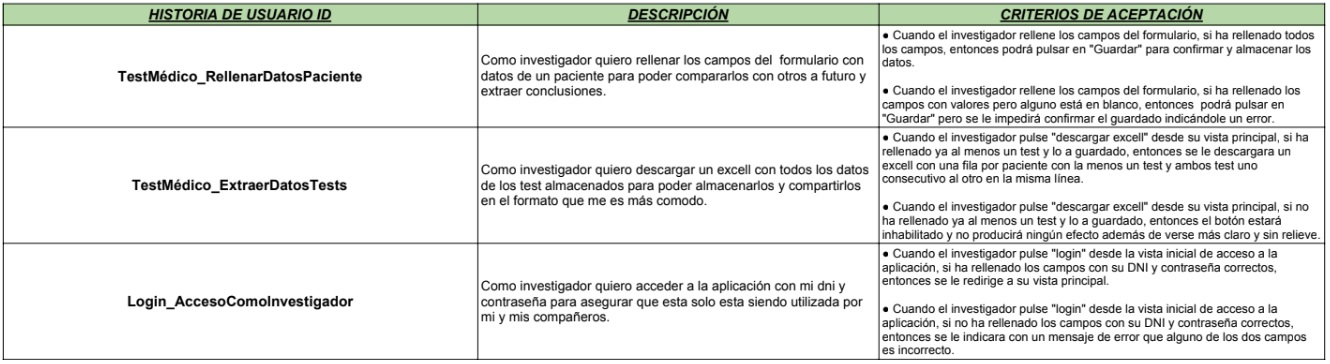
\includegraphics[width=1\textwidth]{images/historiasUsuario-1.jpg}
    \caption{Historias de usuario de mayor importancia, Walking Skeleton de la aplicación.}
\end{figure}
\newpage

Como se puede apreciar en las historias de usuario lo principal es tener unos test donde rellenar los datos de los pacientes de forma cómoda, que estos datos puedan luego ser extraídos en un excel y que el acceso a la aplicación sea privado a los miembros del equipo médico. Las dos primeras suponen la entrada y salida más básica de datos que permitirá al equipo médico extraer sus conclusiones y la tercera, a pesar de ser solo el login, el acceso a la aplicación, es también de gran importancia. Uno de los requisitos principales del estudio es el control de la procedencia y gestión de los datos. Únicamente pacientes que se hayan ofrecido voluntariamente vía formulario pueden tener sus datos representados y solo los miembros oficiales del estudio pueden tener acceso a ellos. Esto se consigue mediante un login cerrado que no permite ningún tipo de registro desde el exterior y la creación de todos los perfiles de investigador manualmente por el administrador.
\newline

El siguiente bloque de funcionalidades complementa las tres primeras que en el primer prototipo emplearían perfiles introducidos a mano en la base de datos para probarse:
\newline

 \begin{figure}[h]
    \centering
     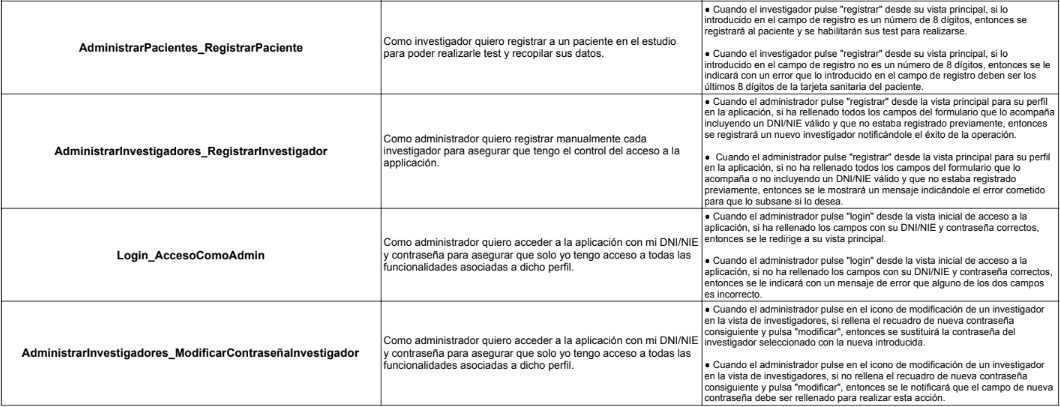
\includegraphics[width=1\textwidth]{images/historiasUsuario-2.jpg}
    \caption{Historias de usuario sobre la inclusión del perfil de administrador y los diversos registros.}
\end{figure}
\newline

En este bloque se recogen los registros tanto de paciente como investigador así como el perfil de administrador y una funcionalidad que quizá sorprenda encontrarse tan pronto en la escala de prioridades, la modificación de contraseñas. Aparentemente por lo explicado de parte del equipo médico es un problema usual la perdida de contraseña o el filtrado de las mismas por las condiciones de su ambiente de trabajo, y tener un acceso cómodo a su modificación es de gran importancia para ellos. Los desarrolladores lo veían mas como algo secundario pero en este artefacto manda el cliente y así es como se recogió.
\newpage

Las funcionalidades que prosiguieron en la escala de valor para el cliente fueron las siguientes:
\newline

 \begin{figure}[h]
    \centering
     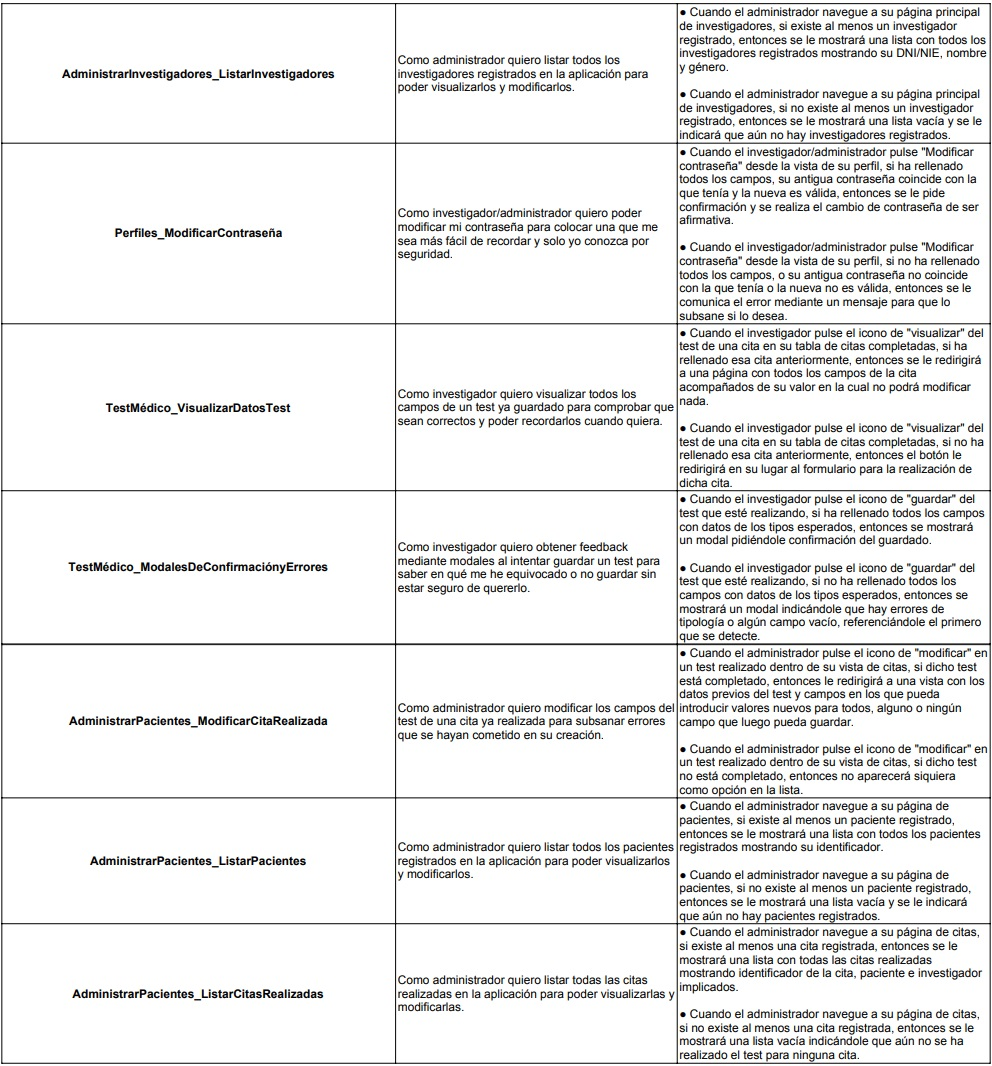
\includegraphics[width=1\textwidth]{images/historiasUsuario-3.jpg}
    \caption{Historias de usuario sobre listado de usuarios y diversas modificaciones.}
\end{figure}
\newline

Estas funcionalidades se componen de dos tablas que listen de forma limpia tanto investigadores para el perfil de administrador como pacientes para el de investigador. La funcionalidad de modificar contraseña de nuevo aparece, pero esta vez es para que cada investigador pueda cambiar su propia clave. Esta funcionalidad es principalmente para que el administrador pueda crear sus perfiles con contraseñas que ellos mismos puedan modificar al obtener las cuentas a algo fácil de recordar para ellos mismos. Además se añade la posibilidad de visualizar es una plantilla los datos de un test realizado, ahorrando tener que extraer el excel y consultarlo cada vez cuando solo se quiere revisar el test de una cita. Se añaden modales para indicar errores y confirmación en los test, importante ya que estos no pueden ser modificados una vez guardados a no ser que lo haga el administrador manualmente. Esta posibilidad de modificar una cita por el administrador es la ultima funcionalidad no comentada de este bloque.

